% Figure (chapter 4): pipeline of the work, from the dataset to the evaluation.
% Compiled by make_all.py with pdflatex; the PDF goes to 07_RELAZIONE/images/schema_pipeline.pdf.
\documentclass[tikz,border=3pt]{standalone}
\usepackage[utf8]{inputenc}
\usepackage[T1]{fontenc}
\usepackage{lmodern}
\usetikzlibrary{arrows.meta,positioning,calc}
\definecolor{dati}{RGB}{42,120,214}
\definecolor{arancio}{RGB}{235,104,52}
\definecolor{verde}{RGB}{27,175,122}
\definecolor{grigio}{RGB}{82,81,78}
\begin{document}
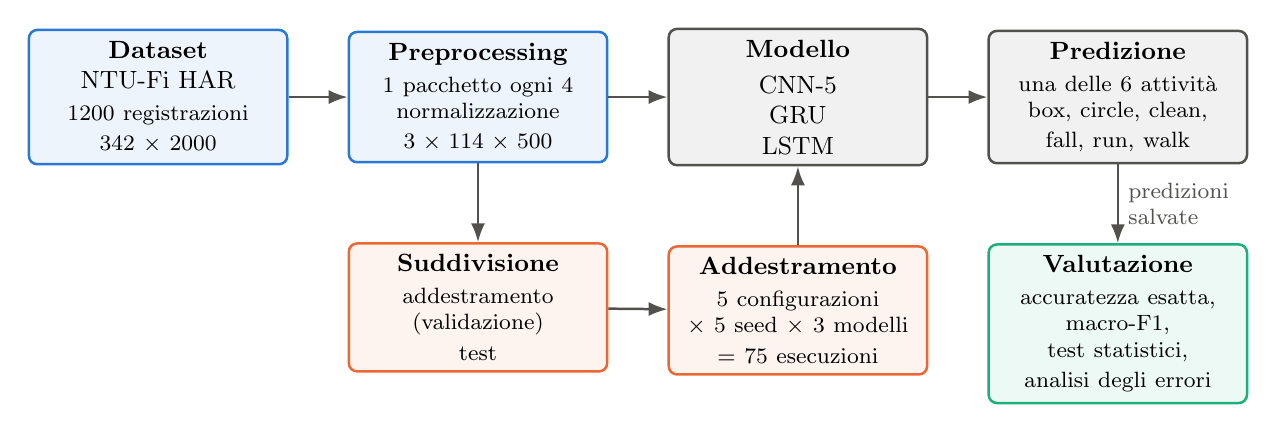
\begin{tikzpicture}[>={Latex[length=2.4mm]}, font=\small,
    box/.style={draw=#1, line width=0.9pt, rounded corners=3pt, fill=#1!8, align=center,
                minimum height=1.55cm, text width=3.0cm, inner sep=4pt},
    box/.default=dati,
    freccia/.style={->, line width=0.9pt, draw=grigio}]

  % riga superiore: il percorso di un campione
  \node[box] (dati) {{\bfseries Dataset}\\NTU-Fi HAR\\[2pt]\footnotesize 1200 registrazioni\\ \footnotesize $342 \times 2000$};
  \node[box, right=0.75cm of dati] (pre) {{\bfseries Preprocessing}\\[2pt]\footnotesize 1 pacchetto ogni 4\\ \footnotesize normalizzazione\\ \footnotesize $3 \times 114 \times 500$};
  \node[box=grigio, right=0.75cm of pre] (mod) {{\bfseries Modello}\\[2pt]CNN-5\\GRU\\LSTM};
  \node[box=grigio, right=0.75cm of mod] (out) {{\bfseries Predizione}\\[2pt]\footnotesize una delle 6 attività\\ \footnotesize box, circle, clean,\\ \footnotesize fall, run, walk};
  \draw[freccia] (dati) -- (pre);
  \draw[freccia] (pre) -- (mod);
  \draw[freccia] (mod) -- (out);

  % riga inferiore: come vengono usati i dati
  \node[box=arancio, below=1.0cm of pre] (split) {{\bfseries Suddivisione}\\[2pt]\footnotesize addestramento\\ \footnotesize (validazione)\\ \footnotesize test};
  \node[box=arancio, below=1.0cm of mod] (train) {{\bfseries Addestramento}\\[2pt]\footnotesize 5 configurazioni\\ \footnotesize $\times$ 5 seed $\times$ 3 modelli\\ \footnotesize = 75 esecuzioni};
  \node[box=verde, below=1.0cm of out] (ana) {{\bfseries Valutazione}\\[2pt]\footnotesize accuratezza esatta,\\ \footnotesize macro-F1, test statistici,\\ \footnotesize analisi degli errori};
  \draw[freccia] (pre) -- (split);
  \draw[freccia] (split) -- (train);
  \draw[freccia] (train) -- (mod);
  \draw[freccia] (out) -- node[right, font=\footnotesize, align=left, text=grigio] {predizioni\\salvate} (ana);
\end{tikzpicture}
\end{document}
